\section{Solution Architecture} \label{sec4}
\noindent
In this section, we explain our solution architecture for schedulability assessment. As described in the previous section,
we are given a set of $n$ control loops, with their bus access states marked as the accepting ones. Recall that our
scheduling objective is to be able to grant bus access infinitely often to each control loop. To check if the system
is safe and schedulable, we carry out the following steps: 

\begin{itemize}

\item We compute the intersection of the individual control loops using the construction explained below. 

\item Once the product is computed, we look for the presence of a cycle that contains at least one state
from each control loop. In other words, on any infinite run of the product automaton, each control loop
repeats infinitely often and is therefore, granted bus access infinitely often as well. \\

\end{itemize}

\begin{definition}Intersection of B\"{u}chi automata~\cite{product}:
\begin{itemize}
 \item Let $B_1 = (\Sigma,Q_1,\Delta_1,{Q_1}^0,F_1)$ and $B_2 = (\Sigma,Q_2,\Delta_2,{Q_2}^0,F_2)$
 \item We can build an automaton for $L(B_1)\footnote{L(name of automaton) represents the language accepted the the automaton}\cap L(B_2)$ as follows
 \item $B_1 \cap B_2 = (\Sigma, Q_1 \times Q_2 \times {0,1,2},\Delta, Q^0_1 \times Q^0_2 \times
       {0}, Q_1 \times Q_2 \times {2})$
 \item We have $(\langle r,q,x \rangle,a,\langle r^{'},q^{'},y \rangle)$ $\in$ $\Delta$ iff the 
       following conditions hold:
        \begin{itemize}
          \item $(r,a,r^{'})$ $\in$ $\Delta_1$ and $ (q,a,q^{'})$ $\in$ $\Delta_2$
          \item The third component depends on the accepting conditions of $B_1$ and $B_2$.
            \begin{itemize}
             \item If $x = 0$ and $r^{'} \epsilon F_1$ then $y = 1$.
             \item If $x = 1$ and $q^{'} \epsilon F_2$ then $y = 2$.
             \item If $x = 2$ then $y = 0$.
             \item Otherwise, $y = x$
            \end{itemize}

        \end{itemize}
 \item The third component essentially guarantees that accepting states from both $B_1$ and
       $B_2$ appear infinitely often. \\
\end{itemize}
\end{definition}

\noindent
Intersection Automaton construction:
\noindent
For the sake of simplicity and ease of illustration, 
we explain the intersection construction in terms of two automata. 
Let us consider the two B\"{u}chi automata P and Q, as shown in Fig.\ref{fig1} and defined by the
conventional five tuple:

$P = \{(p_0,p_1,p_2),(a,b),p_0, Q \times \sum \rightarrow Q,p_2\}$

$Q = \{(q_0,q_1),(a,b),q_0, Q \times \sum \rightarrow Q,q_1\}$ \\

\noindent
From the diagrams given in Fig.\ref{fig1}, we see that the automaton $P$ can accept $(ab){^\omega}$ 
and the $Q$ automaton can accept $(b){^\omega}$. The resulting intersection automaton will accept
$(ab){^\omega}$. \\

\begin{figure}
\begin{center}
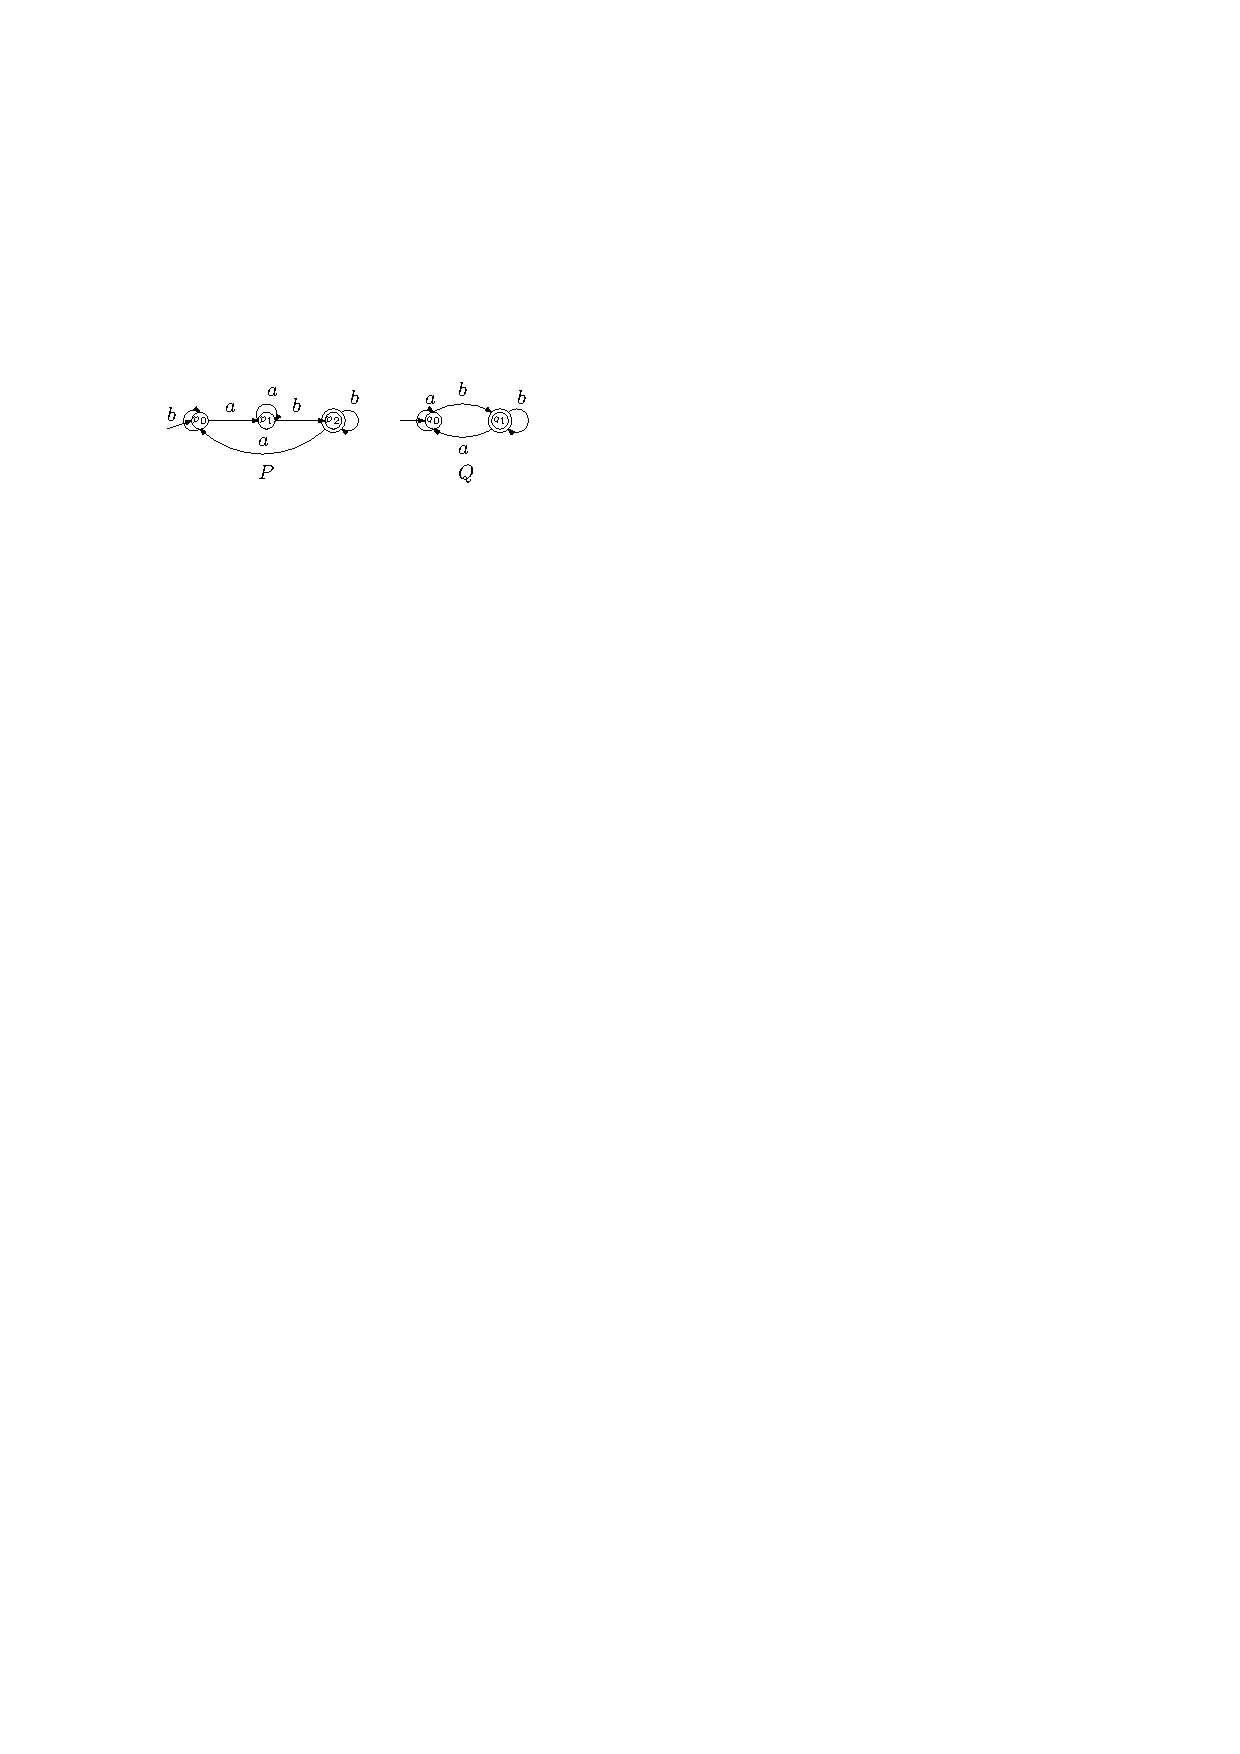
\includegraphics[width=60mm]{example_1.pdf}

%\vspace{-0.1in}
\caption{{\em Individual automata}} \label{fig1}
\end{center}
\end{figure}
 

\noindent
 In the resulting automaton, a cycle is accepted, when it passes through the last copy
 of the product automaton, that signifies the run of the cycle traverses the accepting states of each automaton infinitely often. The remaining cycles, 
 which do not pass through the last copy, are not accepted. We thus augment the classical product construction for finite automata to model our infinitary acceptance requirement.

 
 \begin{figure}
\begin{center}
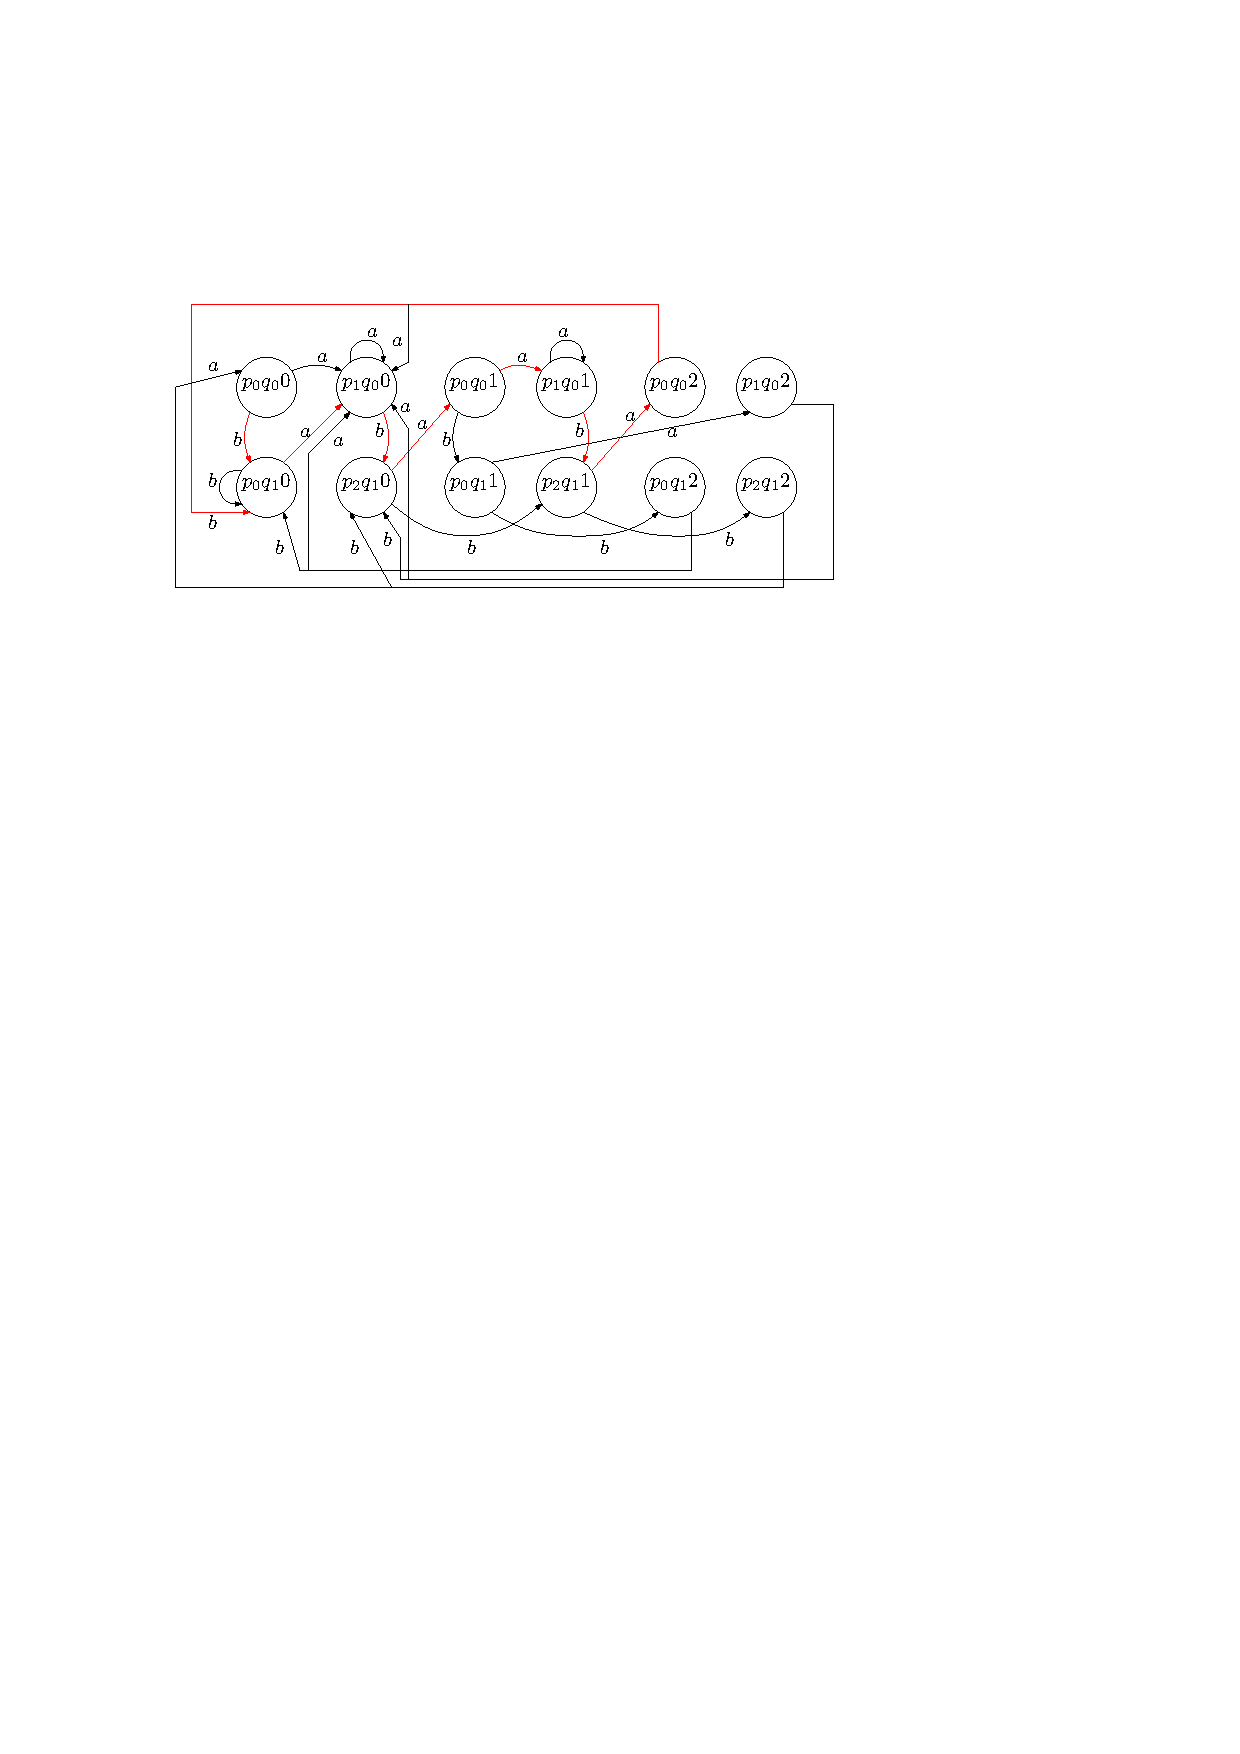
\includegraphics[width=50mm]{state_copy_transition_cycle.pdf}
\end{center}
%\vspace{-0.1in}
\caption{{\em Intersection of the input automata}}
\label{transition}
\end{figure}

\begin{figure}
\begin{center}
%\includegraphics[width=50mm, height=75mm]{algorithn.pdf}
\end{center}
%\vspace{-0.1in}
%\caption{{\em Flow chart of our idea}}
\label{fig:Algorithm}
\end{figure}

\subsection{Verifying the scheduling objective}
\noindent
Once the intersection automaton is constructed, the task of looking for cycles starting from the initial states is carried out.
Cycle detection algorithms are standard in literature~\cite{Clarke:2000:MC:332656} and we implement the same for this work as well. 
Once a cycle is found, we traverse the cycle (every cycle is bound to contain a finite number of states) and check if each control
loop is represented inside it. If not, we proceed to the next cycle and carry out the same check. If all cycles are exhausted and
we do not encounter any one which meets our scheduling objective, we conclude that the schedulability requirement is not met. 
This step is thus quite straightforward. Consider the example given in Figure~\ref{transition}. It can be seen that there are
multiple cycles in the intersection automata, some of which do not contain one representative accepting state from each control 
loop (e.g. $<p0,q0,0> \rightarrow <p1,q0,0> \rightarrow <p1,q0,0>$). Thus it is necessary to examine each cycle to check for
existence of at least one accepting state from each control loop, which is the main idea behind the notion of schedulability we adopt here. 

\subsection{Schedulability violation attack detection}
\noindent
As the system is monitored over time, newer structures of the control loops emerge and we perform the same computation steps
outlined above on the modified structures to check if it remains schedulable even in the presence of the modifications.
Our mechanism can thus be used as a continuous monitor to safe-guard against intermittent control attacks. \\

\noindent
At this onset, we would like to admit that our framework can point out schedulability attacks only. Once the intersection
is computed, we may have 3 different possibilities if schedulability is lost. Assuming that the system was schedulable earlier, 
we may conclude the system has been attacked if any of the following possibilities are detected. Firstly, we may have an empty 
intersection automaton now. As a second possibility, the product may still be non-empty but a cycle may not be reachable.
Finally, a cycle may be found but it may not contain representative tasks from each control loop. All these are indicators of 
schedulability loss according to our analysis method and we conclude that an attack has been carried out.